\documentclass[12pt]{amsart}
\usepackage{fullpage}
\usepackage{pbox}
\usepackage{graphicx}
\usepackage{booktabs} % Top and bottom rules for table
\usepackage{amsfonts, amsmath, amsthm, amssymb}
\usepackage{longtable,array,color,xcolor}
\usepackage[colorlinks = true,
            urlcolor  = blue]{hyperref}
\usepackage{verbatim}
\usepackage{enumerate}
\usepackage{lscape}
\newcommand\narrowstyle{\SetTracking{encoding=*}{-50}\lsstyle}

\setlength{\parindent}{0pt}

\begin{document}
\flushright
Name:\underline{\hspace{5cm}}
\title{Math 320: Quiz 3}
\maketitle

\begin{enumerate}
\item (3 points) Let $f(x) = x^3-7$. Suppose we would
like to find a root of $f(x)$ in the interval $(0,2)$ using the
two endpoints as our ``bracket.''

\begin{enumerate}
\item What are the first two points selected inside the 
interval using the bisection method? Justify your response.

\item How many iterations of the bisection method must be performed
to guarantee error less than or equal to $2^{-16}$?

\item What is the first point inside the interval selected by
the false position (regula falsi) method?
\end{enumerate}

\vfill

\pagebreak

\item (4 points) Let $f(x) = (x^2-1)e^{-x^2}$ be our function of
interest, with graph shown below. 

\centerline{
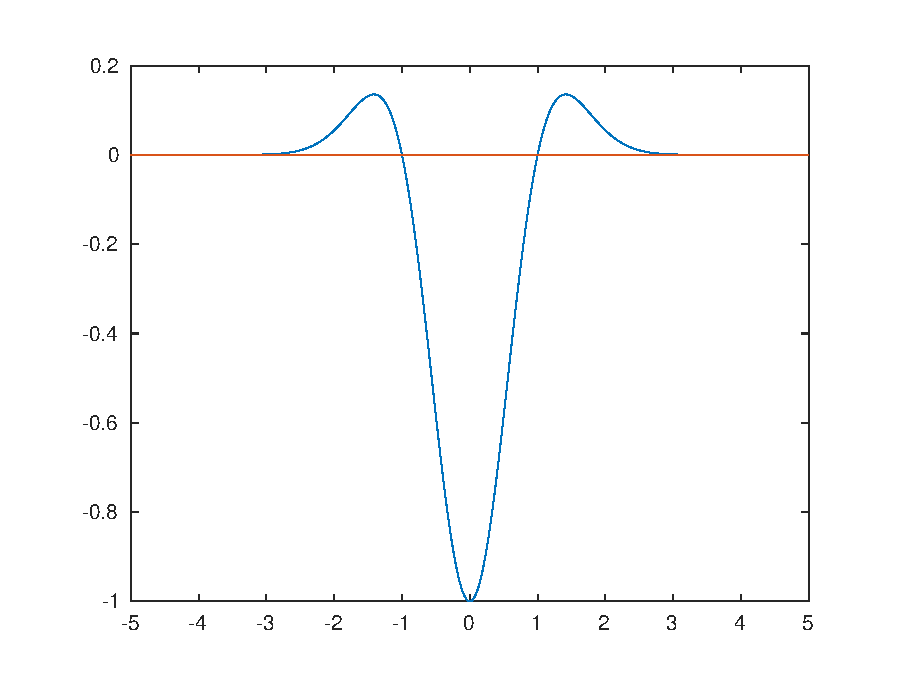
\includegraphics[scale=.6]{q3p2.eps}
}
Suppose we try to find a root using Newton's method.

\begin{enumerate}
\item Compute $f'(x)$.

\item Describe (without actually computing) our approximations by
Newton's method if our initial guess is $x = -2$.


\item Describe  (without actually computing) our approximations by
Newton's method if our initial guess is $x = -1/2$.

\end{enumerate}

\pagebreak
\begin{landscape}
\item (3 points) For the image below, draw and label
secant lines and values for $x_2,x_3$, and $x_4$ given 
$x_0$ and $x_1$ shown here. 

\centerline{
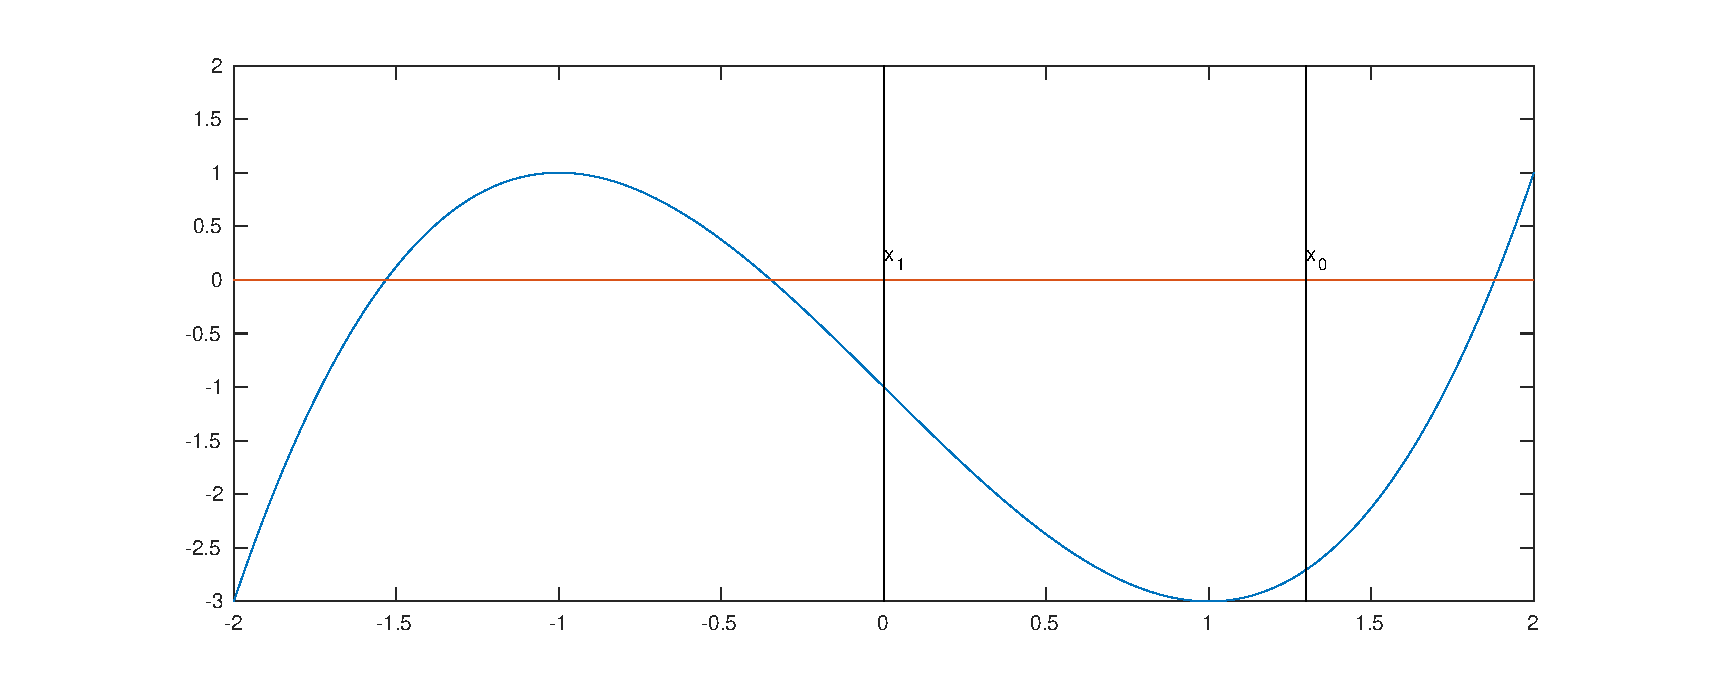
\includegraphics[scale=.8]{q3p3.eps}
}
\end{landscape}
\end{enumerate}

\end{document}
